\documentclass[border=4pt]{standalone}
\usepackage{amsmath,amssymb}
\usepackage{tikz}
\usetikzlibrary{arrows.meta,decorations.pathreplacing,patterns,calc,positioning,shapes.geometric}
\usepackage{pgfplots}
\pgfplotsset{compat=newest}
\begin{document}
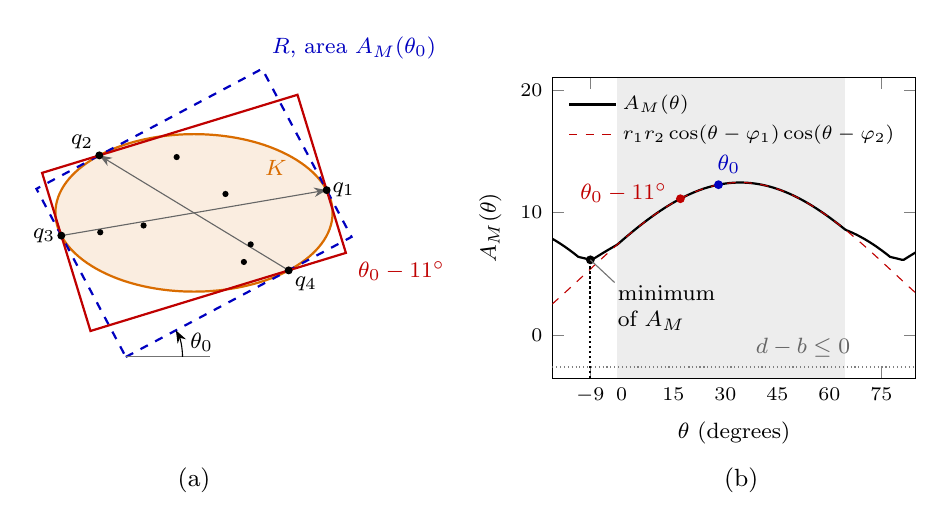
\begin{tikzpicture}[>={Stealth[length=1.6mm]},
  lab/.style={font=\footnotesize},
  ext/.style={thin,black!55}]
%======================== (a) geometry of the proof
\begin{scope}[scale=0.8]
  \colorlet{colK}{orange!85!black}
  \fill[colK!12] (0,0) ellipse [x radius=2.2,y radius=1.25];
  \draw[colK,thick] (0,0) ellipse [x radius=2.2,y radius=1.25];
  % rectangle R at theta_0 = 28 deg, supporting K at q_1,...,q_4
  \draw[blue!75!black,thick,dashed] (-1.082,-2.287) -- (2.501,-0.382) -- (1.082,2.287) -- (-2.501,0.382) -- cycle;
  % rectangle at theta_0 - 11 deg with the same extreme points
  \draw[red!75!black,thick] (-1.643,-1.875) -- (2.411,-0.635) -- (1.643,1.875) -- (-2.411,0.635) -- cycle;
  % vectors q_1 - q_3 and q_2 - q_4
  \draw[->,black!60] (-2.106,-0.361) -- (2.106,0.361);
  \draw[->,black!60] (1.503,-0.913) -- (-1.503,0.913);
  % points of M
  \foreach \p in {(-0.275,0.886),(-1.488,-0.308),(0.792,-0.779),(0.500,0.300),(-0.800,-0.200),(0.900,-0.500)} \fill \p circle (1.4pt);
  \foreach \p/\n/\a in {(2.106,0.361)/q_1/west,(-1.503,0.913)/q_2/south east,(-2.106,-0.361)/q_3/east,(1.503,-0.913)/q_4/north west}
    {\fill \p circle (1.8pt); \node[lab,anchor=\a,inner sep=2pt] at \p {$\n$};}
  % frame of R
  \draw[ext] (-1.082,-2.287) -- (0.25,-2.287);
  \draw[->,thin] (-0.182,-2.287) arc[start angle=0,end angle=28,radius=0.9];
  \node[lab] at (0.12,-2.06) {$\theta_0$};
  \node[lab,colK] at (1.3,0.72) {$K$};
  \node[lab,blue!75!black,anchor=south west] at (1.082,2.287) {$R$, area $A_M(\theta_0)$};
  \node[lab,red!75!black,anchor=north west] at (2.45,-0.62) {$\theta_0-11^\circ$};
  \node[font=\small] at (0,-4.25) {(a)};
\end{scope}
%======================== (b) area function of M
\begin{scope}[xshift=4.55cm,yshift=-2.1cm]
\begin{axis}[width=6.2cm,height=5.4cm,
  xmin=-20,xmax=85,ymin=-3.5,ymax=21,
  xtick={-9,0,15,30,45,60,75},
  xlabel={$\theta$ (degrees)},ylabel={$A_M(\theta)$},
  label style={font=\footnotesize},tick label style={font=\scriptsize},
  legend style={font=\scriptsize,at={(0.98,0.98)},anchor=north east,draw=none,fill=none},
  legend cell align=left]
  \fill[black!7] (axis cs:-1.2,-3.5) rectangle (axis cs:64.6,21);
  \addplot[black,thick] coordinates {(-20.0,7.867) (-19.5,7.784) (-19.0,7.700) (-18.5,7.613) (-18.0,7.524) (-17.5,7.432) (-17.0,7.339) (-16.5,7.243) (-16.0,7.145) (-15.5,7.044) (-15.0,6.942) (-14.5,6.837) (-14.0,6.730) (-13.5,6.622) (-13.0,6.511) (-12.5,6.398) (-12.0,6.356) (-11.5,6.325) (-11.0,6.292) (-10.5,6.258) (-10.0,6.222) (-9.5,6.185) (-9.0,6.147) (-8.5,6.155) (-8.0,6.244) (-7.5,6.333) (-7.0,6.421) (-6.5,6.508) (-6.0,6.595) (-5.5,6.681) (-5.0,6.766) (-4.5,6.851) (-4.0,6.935) (-3.5,7.018) (-3.0,7.101) (-2.5,7.182) (-2.0,7.263) (-1.5,7.343) (-1.0,7.443) (-0.5,7.566) (0.0,7.688) (0.5,7.810) (1.0,7.931) (1.5,8.051) (2.0,8.169) (2.5,8.287) (3.0,8.404) (3.5,8.520) (4.0,8.635) (4.5,8.748) (5.0,8.861) (5.5,8.972) (6.0,9.082) (6.5,9.191) (7.0,9.298) (7.5,9.404) (8.0,9.509) (8.5,9.612) (9.0,9.714) (9.5,9.814) (10.0,9.913) (10.5,10.011) (11.0,10.107) (11.5,10.201) (12.0,10.294) (12.5,10.385) (13.0,10.474) (13.5,10.562) (14.0,10.648) (14.5,10.732) (15.0,10.815) (15.5,10.895) (16.0,10.974) (16.5,11.051) (17.0,11.127) (17.5,11.200) (18.0,11.271) (18.5,11.341) (19.0,11.408) (19.5,11.474) (20.0,11.537) (20.5,11.599) (21.0,11.658) (21.5,11.716) (22.0,11.771) (22.5,11.825) (23.0,11.876) (23.5,11.925) (24.0,11.972) (24.5,12.017) (25.0,12.059) (25.5,12.100) (26.0,12.138) (26.5,12.174) (27.0,12.208) (27.5,12.240) (28.0,12.269) (28.5,12.296) (29.0,12.321) (29.5,12.344) (30.0,12.365) (30.5,12.383) (31.0,12.399) (31.5,12.412) (32.0,12.424) (32.5,12.433) (33.0,12.440) (33.5,12.444) (34.0,12.446) (34.5,12.446) (35.0,12.444) (35.5,12.439) (36.0,12.432) (36.5,12.423) (37.0,12.412) (37.5,12.398) (38.0,12.382) (38.5,12.364) (39.0,12.343) (39.5,12.320) (40.0,12.295) (40.5,12.268) (41.0,12.238) (41.5,12.206) (42.0,12.172) (42.5,12.136) (43.0,12.098) (43.5,12.057) (44.0,12.014) (44.5,11.970) (45.0,11.922) (45.5,11.873) (46.0,11.822) (46.5,11.769) (47.0,11.713) (47.5,11.656) (48.0,11.596) (48.5,11.534) (49.0,11.471) (49.5,11.405) (50.0,11.337) (50.5,11.268) (51.0,11.196) (51.5,11.123) (52.0,11.048) (52.5,10.971) (53.0,10.892) (53.5,10.811) (54.0,10.728) (54.5,10.644) (55.0,10.558) (55.5,10.470) (56.0,10.380) (56.5,10.289) (57.0,10.197) (57.5,10.102) (58.0,10.006) (58.5,9.909) (59.0,9.810) (59.5,9.709) (60.0,9.607) (60.5,9.504) (61.0,9.399) (61.5,9.293) (62.0,9.185) (62.5,9.077) (63.0,8.966) (63.5,8.855) (64.0,8.743) (64.5,8.629) (65.0,8.552) (65.5,8.495) (66.0,8.435) (66.5,8.373) (67.0,8.308) (67.5,8.241) (68.0,8.171) (68.5,8.099) (69.0,8.024) (69.5,7.946) (70.0,7.867) (70.5,7.784) (71.0,7.700) (71.5,7.613) (72.0,7.524) (72.5,7.432) (73.0,7.339) (73.5,7.243) (74.0,7.145) (74.5,7.044) (75.0,6.942) (75.5,6.837) (76.0,6.730) (76.5,6.622) (77.0,6.511) (77.5,6.398) (78.0,6.356) (78.5,6.325) (79.0,6.292) (79.5,6.258) (80.0,6.222) (80.5,6.185) (81.0,6.147) (81.5,6.155) (82.0,6.244) (82.5,6.333) (83.0,6.421) (83.5,6.508) (84.0,6.595) (84.5,6.681) (85.0,6.766)};
  \addlegendentry{$A_M(\theta)$}
  \addplot[red!75!black,dashed] coordinates {(-20.0,2.549) (-19.5,2.674) (-19.0,2.800) (-18.5,2.926) (-18.0,3.052) (-17.5,3.180) (-17.0,3.308) (-16.5,3.436) (-16.0,3.565) (-15.5,3.694) (-15.0,3.823) (-14.5,3.953) (-14.0,4.083) (-13.5,4.214) (-13.0,4.345) (-12.5,4.475) (-12.0,4.606) (-11.5,4.738) (-11.0,4.869) (-10.5,5.000) (-10.0,5.131) (-9.5,5.262) (-9.0,5.393) (-8.5,5.524) (-8.0,5.655) (-7.5,5.785) (-7.0,5.915) (-6.5,6.045) (-6.0,6.175) (-5.5,6.304) (-5.0,6.433) (-4.5,6.561) (-4.0,6.689) (-3.5,6.816) (-3.0,6.943) (-2.5,7.069) (-2.0,7.194) (-1.5,7.319) (-1.0,7.443) (-0.5,7.566) (0.0,7.688) (0.5,7.810) (1.0,7.931) (1.5,8.051) (2.0,8.169) (2.5,8.287) (3.0,8.404) (3.5,8.520) (4.0,8.635) (4.5,8.748) (5.0,8.861) (5.5,8.972) (6.0,9.082) (6.5,9.191) (7.0,9.298) (7.5,9.404) (8.0,9.509) (8.5,9.612) (9.0,9.714) (9.5,9.814) (10.0,9.913) (10.5,10.011) (11.0,10.107) (11.5,10.201) (12.0,10.294) (12.5,10.385) (13.0,10.474) (13.5,10.562) (14.0,10.648) (14.5,10.732) (15.0,10.815) (15.5,10.895) (16.0,10.974) (16.5,11.051) (17.0,11.127) (17.5,11.200) (18.0,11.271) (18.5,11.341) (19.0,11.408) (19.5,11.474) (20.0,11.537) (20.5,11.599) (21.0,11.658) (21.5,11.716) (22.0,11.771) (22.5,11.825) (23.0,11.876) (23.5,11.925) (24.0,11.972) (24.5,12.017) (25.0,12.059) (25.5,12.100) (26.0,12.138) (26.5,12.174) (27.0,12.208) (27.5,12.240) (28.0,12.269) (28.5,12.296) (29.0,12.321) (29.5,12.344) (30.0,12.365) (30.5,12.383) (31.0,12.399) (31.5,12.412) (32.0,12.424) (32.5,12.433) (33.0,12.440) (33.5,12.444) (34.0,12.446) (34.5,12.446) (35.0,12.444) (35.5,12.439) (36.0,12.432) (36.5,12.423) (37.0,12.412) (37.5,12.398) (38.0,12.382) (38.5,12.364) (39.0,12.343) (39.5,12.320) (40.0,12.295) (40.5,12.268) (41.0,12.238) (41.5,12.206) (42.0,12.172) (42.5,12.136) (43.0,12.098) (43.5,12.057) (44.0,12.014) (44.5,11.970) (45.0,11.922) (45.5,11.873) (46.0,11.822) (46.5,11.769) (47.0,11.713) (47.5,11.656) (48.0,11.596) (48.5,11.534) (49.0,11.471) (49.5,11.405) (50.0,11.337) (50.5,11.268) (51.0,11.196) (51.5,11.123) (52.0,11.048) (52.5,10.971) (53.0,10.892) (53.5,10.811) (54.0,10.728) (54.5,10.644) (55.0,10.558) (55.5,10.470) (56.0,10.380) (56.5,10.289) (57.0,10.197) (57.5,10.102) (58.0,10.006) (58.5,9.909) (59.0,9.810) (59.5,9.709) (60.0,9.607) (60.5,9.504) (61.0,9.399) (61.5,9.293) (62.0,9.185) (62.5,9.077) (63.0,8.966) (63.5,8.855) (64.0,8.743) (64.5,8.629) (65.0,8.514) (65.5,8.399) (66.0,8.282) (66.5,8.164) (67.0,8.045) (67.5,7.925) (68.0,7.804) (68.5,7.683) (69.0,7.560) (69.5,7.437) (70.0,7.313) (70.5,7.188) (71.0,7.063) (71.5,6.936) (72.0,6.810) (72.5,6.682) (73.0,6.555) (73.5,6.426) (74.0,6.298) (74.5,6.168) (75.0,6.039) (75.5,5.909) (76.0,5.779) (76.5,5.648) (77.0,5.518) (77.5,5.387) (78.0,5.256) (78.5,5.125) (79.0,4.993) (79.5,4.862) (80.0,4.731) (80.5,4.600) (81.0,4.469) (81.5,4.338) (82.0,4.208) (82.5,4.077) (83.0,3.947) (83.5,3.817) (84.0,3.688) (84.5,3.558) (85.0,3.430)};
  \addlegendentry{$r_1r_2\cos(\theta-\varphi_1)\cos(\theta-\varphi_2)$}
  \addplot[black!50,densely dotted,domain=-20:85] {-2.584};
  \fill[blue!75!black] (axis cs:28,12.269) circle (1.6pt);
  \fill[red!75!black] (axis cs:17,11.127) circle (1.6pt);
  \draw[densely dotted,thick] (axis cs:-9,-3.5) -- (axis cs:-9,6.147);
  \fill (axis cs:-9,6.147) circle (1.6pt);
  \node[lab,anchor=south,blue!75!black] at (axis cs:31,12.4) {$\theta_0$};
  \node[lab,anchor=east,red!75!black] at (axis cs:16,11.6) {$\theta_0-11^\circ$};
  \draw[ext] (axis cs:-9,6.147) -- (axis cs:-2,4.3) node[lab,black,anchor=north west,inner sep=1pt,align=left] {minimum\\of $A_M$};
  \node[lab,anchor=south west,black!60] at (axis cs:36,-2.55) {$d-b\le0$};
\end{axis}
\node[font=\small] at (2.4,-1.3) {(b)};
\end{scope}
\end{tikzpicture}
\end{document}
